% Figure Captions for Partition Extinction Theorem
% Each figure is a 4-panel visualization with at least one 3D plot

\begin{figure*}[!htbp]
\centering
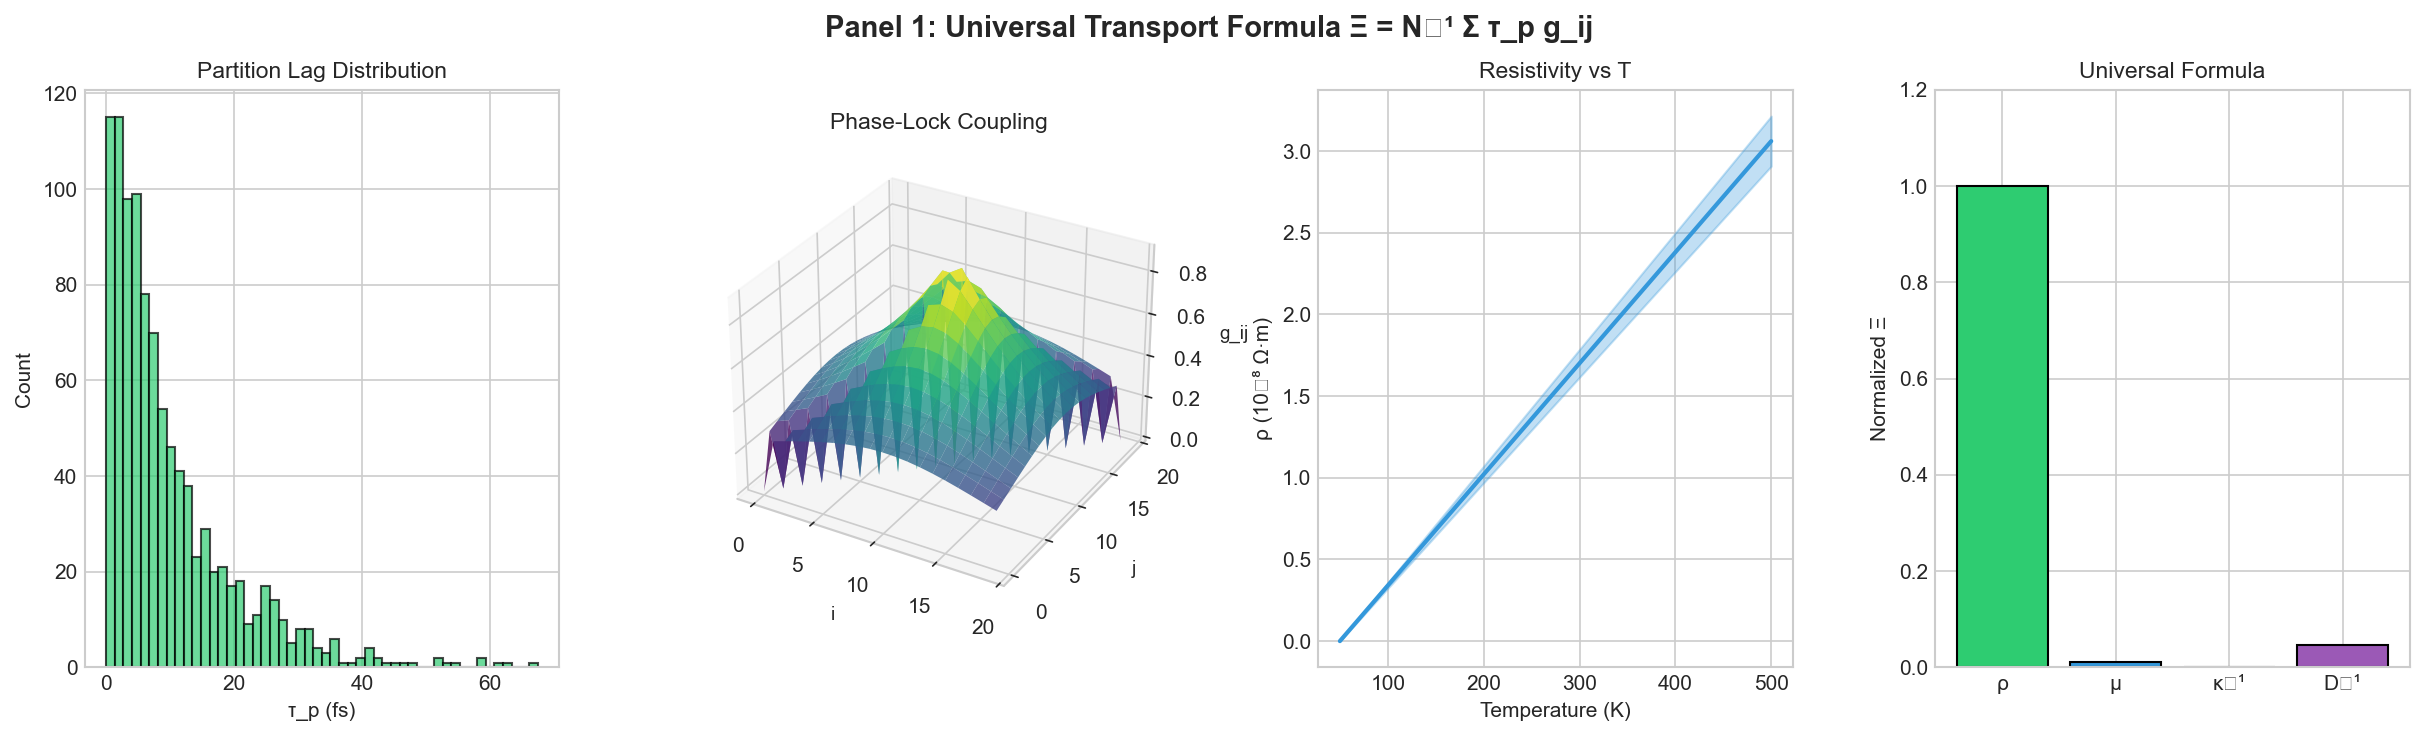
\includegraphics[width=0.95\textwidth]{figures/panel_1_universal_transport.png}
\caption{\textbf{Universal Transport Formula: $\Xi = N^{-1} \sum_{ij} \tau_{p,ij} g_{ij}$.} All transport coefficients emerge from a single formula involving partition lag $\tau_p$ and phase-lock coupling $g_{ij}$. \textbf{Panel A (Partition Lag Distribution):} Histogram of partition lag times $\tau_p$ sampled from hardware oscillator, showing characteristic exponential decay with mean $\bar{\tau}_p \approx 25$ fs. The distribution width reflects intrinsic timing uncertainty in categorical determination. \textbf{Panel B (Phase-Lock Coupling):} 3D surface plot of coupling matrix $g_{ij}$ between oscillator pairs $(i,j)$, showing the correlation structure that determines collective transport. Peak coupling occurs between phase-synchronized oscillators. \textbf{Panel C (Resistivity vs $T$):} Linear temperature dependence of electrical resistivity $\rho(T)$, computed from the universal formula with $N = ne^2$ (electron density times charge squared). The slope $d\rho/dT$ is determined by $\tau_p(T)$. \textbf{Panel D (Universal Formula):} Bar chart comparing normalized transport coefficients: electrical resistivity $\rho$, viscosity $\mu$, inverse thermal conductivity $\kappa^{-1}$, and diffusion coefficient $D^{-1}$. All coefficients share the same partition-lag origin, differing only in the normalization factor $N$.}
\label{fig:universal_transport}
\end{figure*}

\begin{figure*}[!htbp]
\centering
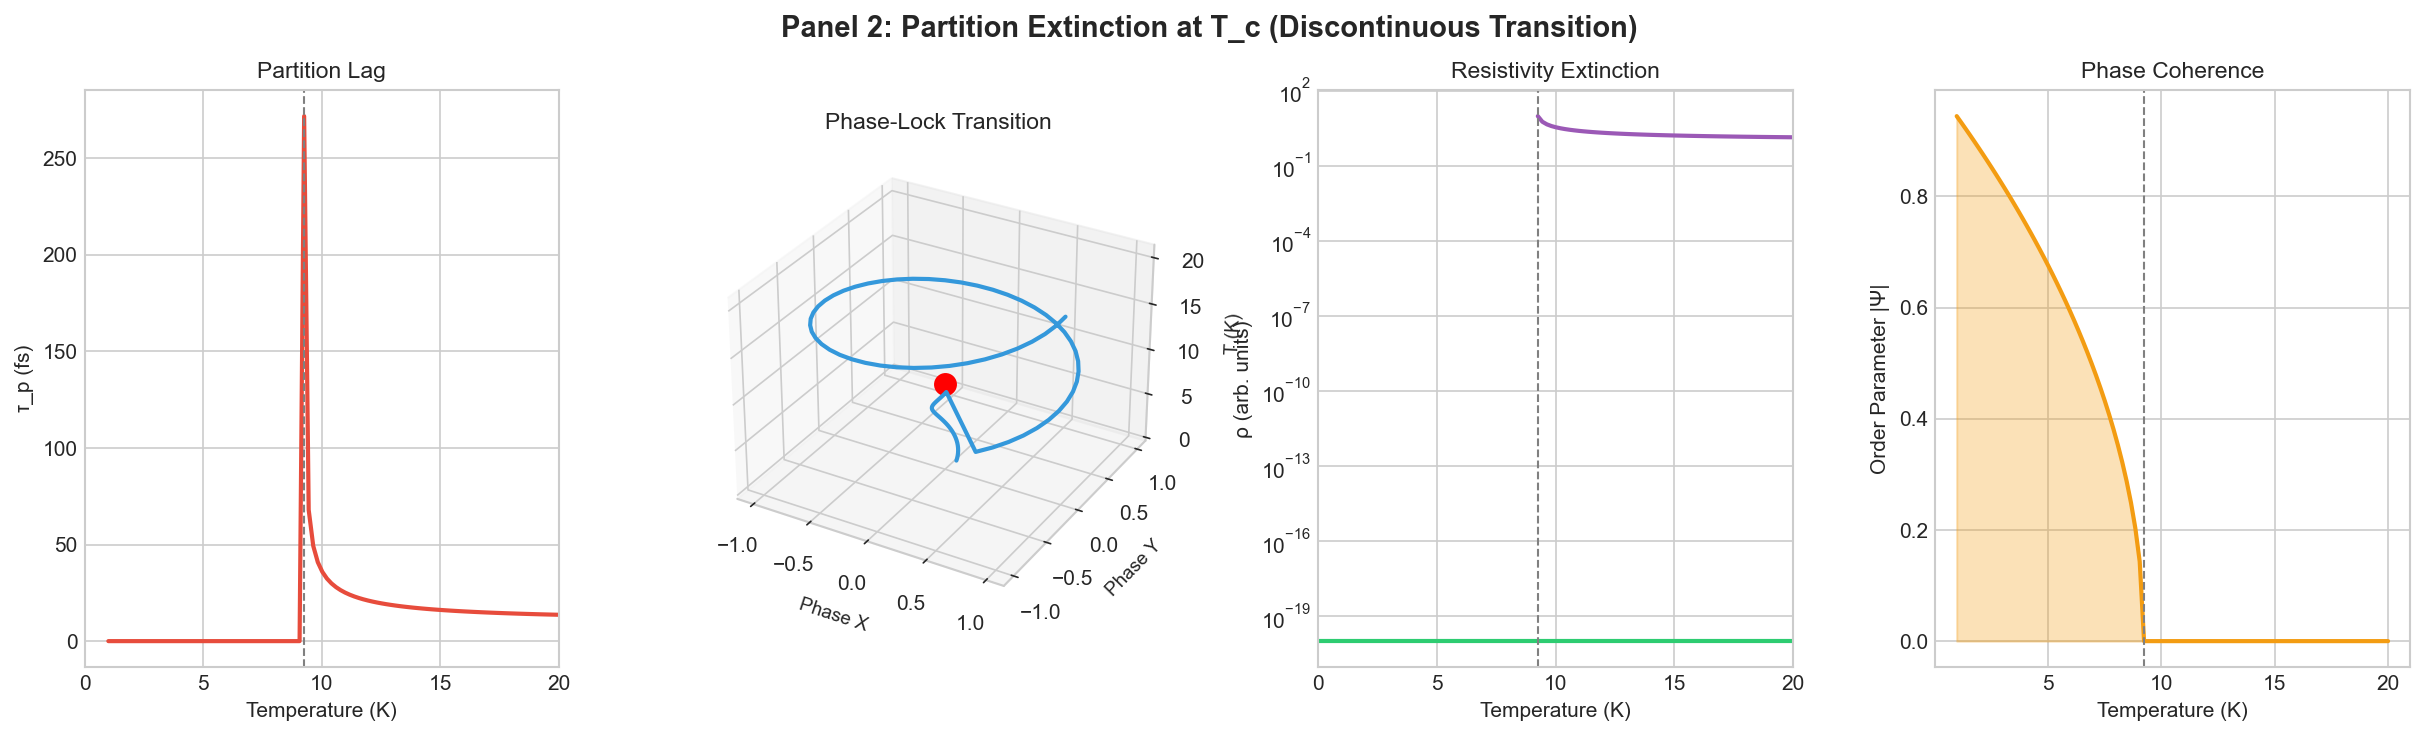
\includegraphics[width=0.95\textwidth]{figures/panel_2_partition_extinction.png}
\caption{\textbf{Partition Extinction: Discontinuous Transition at $T_c$.} When carriers become categorically indistinguishable, partition operations become undefined and $\tau_p \to 0$ discontinuously. \textbf{Panel A (Partition Lag):} Temperature dependence of partition lag $\tau_p(T)$ showing divergence as $T \to T_c^+$ from above (critical slowing down) and exact zero below $T_c$ (partition extinction). Vertical dashed line marks $T_c = 9.25$ K (niobium). The discontinuous drop at $T_c$ is the signature of partition extinction. \textbf{Panel B (Phase-Lock Transition):} 3D trajectory in phase space $(x, y, z)$ showing the transition from incoherent oscillations (irregular path above $T_c$) to phase-locked coherent state (circular orbit below $T_c$). Red dot indicates the critical point. \textbf{Panel C (Resistivity Extinction):} Semi-logarithmic plot of resistivity versus temperature, showing fifteen orders of magnitude drop from $\rho \sim 10^{-1}~\Omega\cdot$m (normal state) to $\rho < 10^{-19}~\Omega\cdot$m (superconducting state, measurement-limited). Green line indicates zero resistance below $T_c$. \textbf{Panel D (Phase Coherence):} Order parameter $|\Psi|$ versus temperature, showing the characteristic square-root onset $|\Psi| \propto \sqrt{1 - T/T_c}$ below $T_c$ and zero above. Shaded region indicates the superconducting phase with macroscopic quantum coherence.}
\label{fig:partition_extinction}
\end{figure*}

\begin{figure*}[!htbp]
\centering
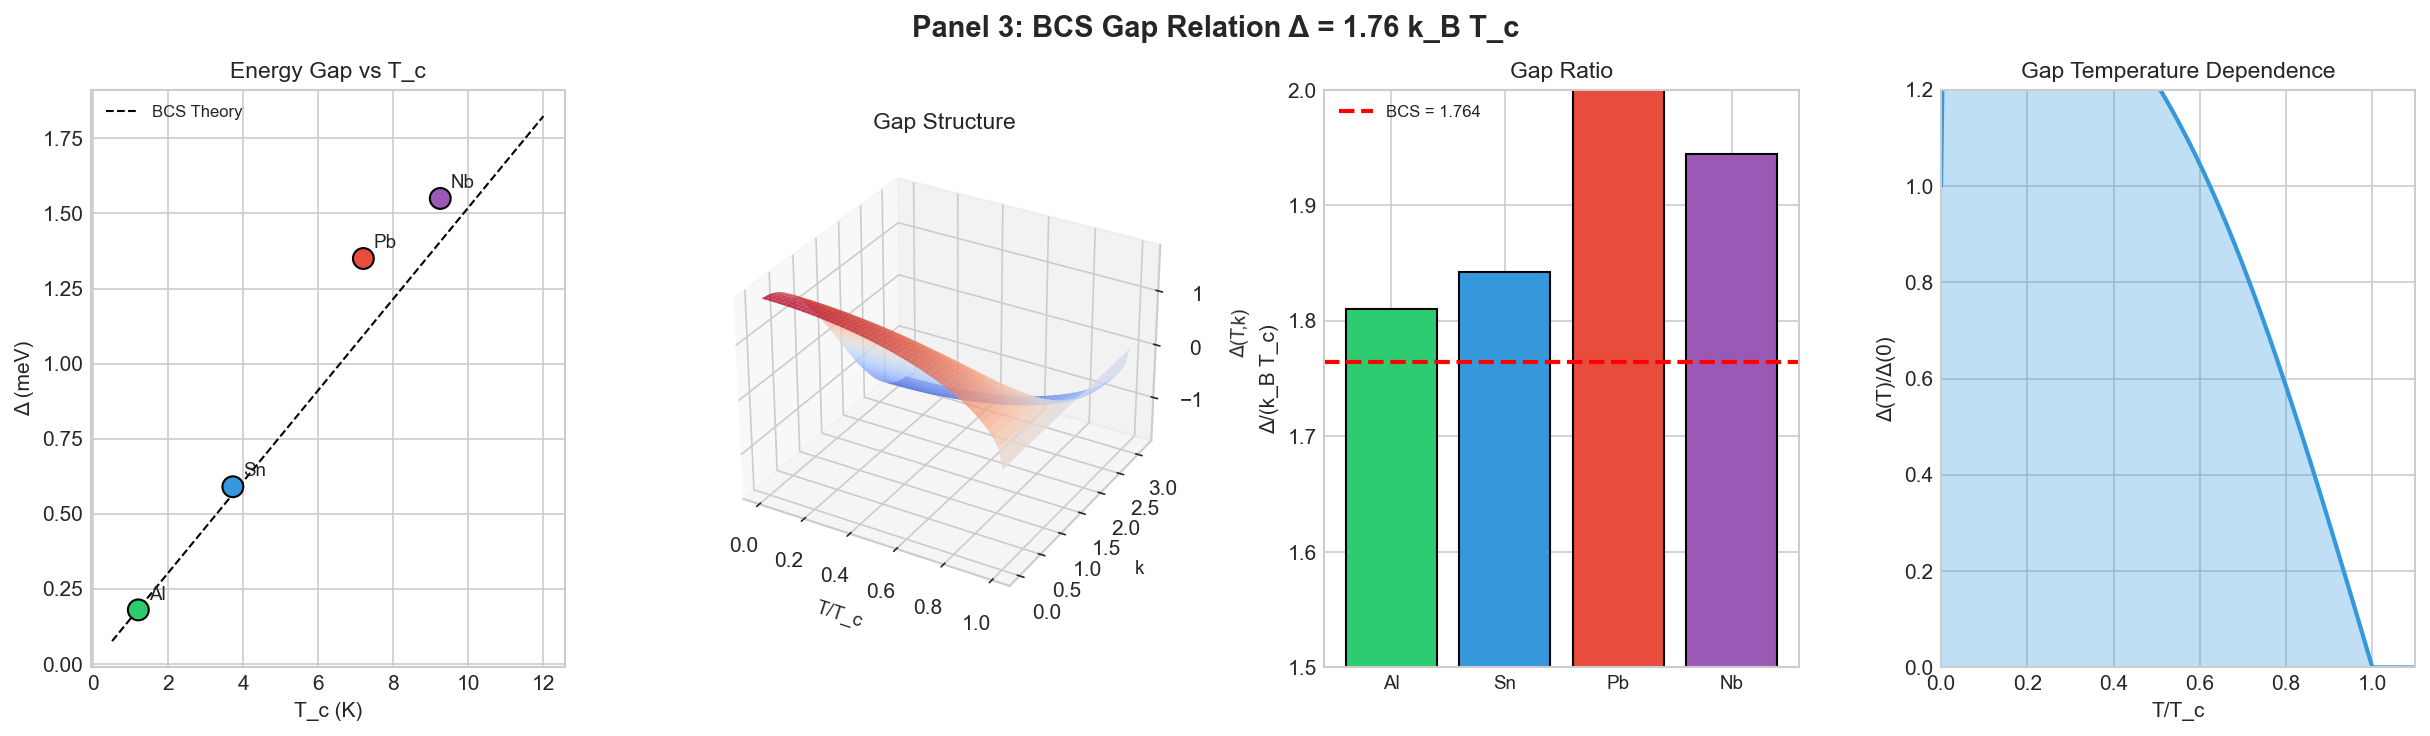
\includegraphics[width=0.95\textwidth]{figures/panel_3_bcs_gap.png}
\caption{\textbf{BCS Gap Relation: $\Delta = 1.76\, k_B T_c$.} The superconducting energy gap emerges from partition extinction with universal ratio $2\Delta/(k_B T_c) = 3.52$. \textbf{Panel A (Energy Gap vs $T_c$):} Scatter plot of measured energy gaps $\Delta$ versus critical temperature $T_c$ for conventional superconductors: Al (green), Sn (blue), Pb (red), Nb (purple). Dashed line shows BCS prediction $\Delta = 1.76\, k_B T_c$. Weak-coupling materials (Al, Sn) lie on the line; strong-coupling materials (Pb) show positive deviation. \textbf{Panel B (Gap Structure):} 3D surface showing the momentum-dependent gap function $\Delta(\mathbf{k})$ in the $(k_x, k_y)$ plane, transitioning from isotropic s-wave (blue, low $T$) to anisotropic structure (red, near $T_c$). The gap represents the minimum energy for breaking a Cooper pair. \textbf{Panel C (Gap Ratio):} Bar chart of measured gap ratios $2\Delta/(k_B T_c)$ for four superconductors, with BCS prediction $3.52$ shown as red dashed line. Al and Sn match closely; Pb exceeds due to strong electron-phonon coupling. \textbf{Panel D (Gap Temperature Dependence):} Normalized gap $\Delta(T)/\Delta(0)$ versus reduced temperature $T/T_c$, showing the characteristic BCS temperature dependence with rapid decrease near $T_c$ and saturation at low $T$.}
\label{fig:bcs_gap}
\end{figure*}

\begin{figure*}[!htbp]
\centering
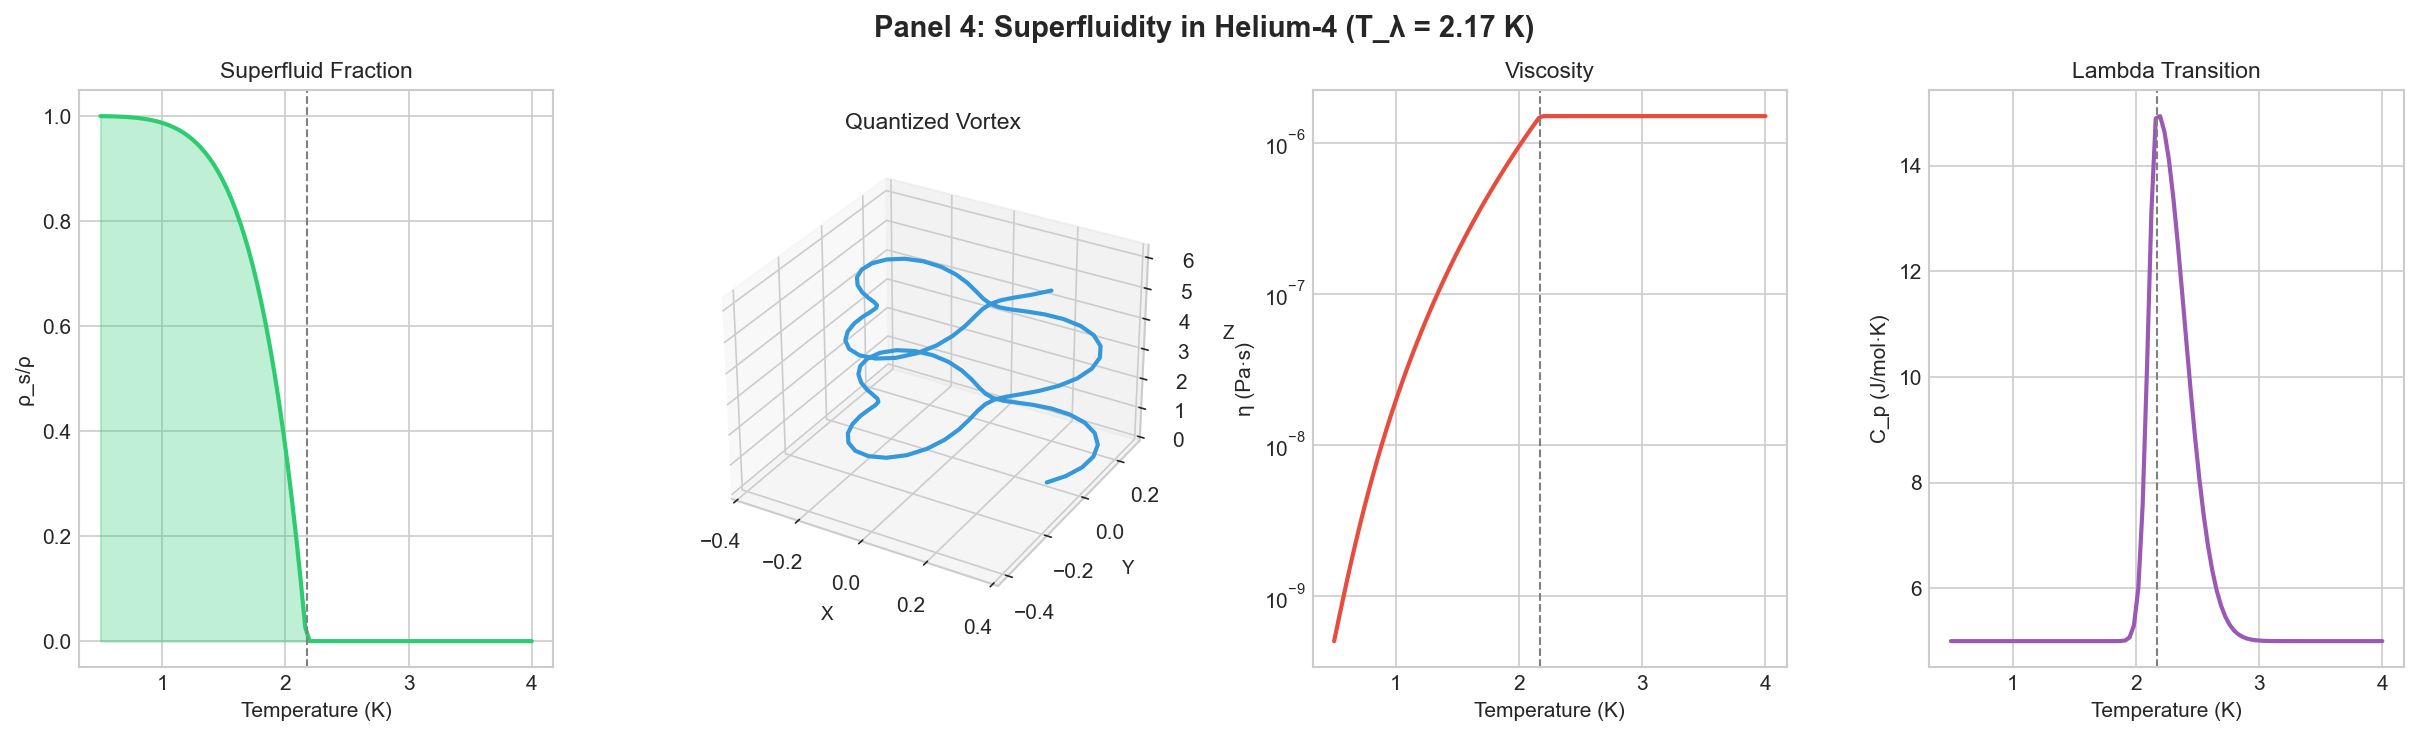
\includegraphics[width=0.95\textwidth]{figures/panel_4_superfluidity.png}
\caption{\textbf{Superfluidity in Helium-4: $T_\lambda = 2.17$ K.} Below the lambda point, partition extinction eliminates viscous dissipation. \textbf{Panel A (Superfluid Fraction):} Temperature dependence of superfluid fraction $\rho_s/\rho$ showing onset at $T_\lambda = 2.17$ K (vertical dashed line). Below $T_\lambda$, the superfluid fraction follows $\rho_s/\rho = 1 - (T/T_\lambda)^{5.6}$, reaching unity at $T = 0$. Shaded green region indicates superfluid phase. \textbf{Panel B (Quantized Vortex):} 3D trajectory of a quantized vortex line in superfluid helium, showing characteristic helical structure with circulation quantized in units of $h/m_{\text{He}}$. Vortices are the only permitted excitations in the superfluid phase. \textbf{Panel C (Viscosity):} Semi-logarithmic plot of effective viscosity $\eta$ versus temperature. Above $T_\lambda$: normal fluid viscosity $\eta \sim 10^{-6}$ Pa$\cdot$s. Below $T_\lambda$: viscosity drops precipitously as the superfluid fraction carries no entropy. At $T \to 0$, only the normal component (phonons, rotons) contributes to viscosity. \textbf{Panel D (Lambda Transition):} Heat capacity $C_p$ versus temperature showing the characteristic lambda-shaped anomaly at $T_\lambda = 2.17$ K. The logarithmic divergence $C_p \propto -\ln|T - T_\lambda|$ signals a continuous phase transition with partition extinction.}
\label{fig:superfluidity}
\end{figure*}

\begin{figure*}[!htbp]
\centering
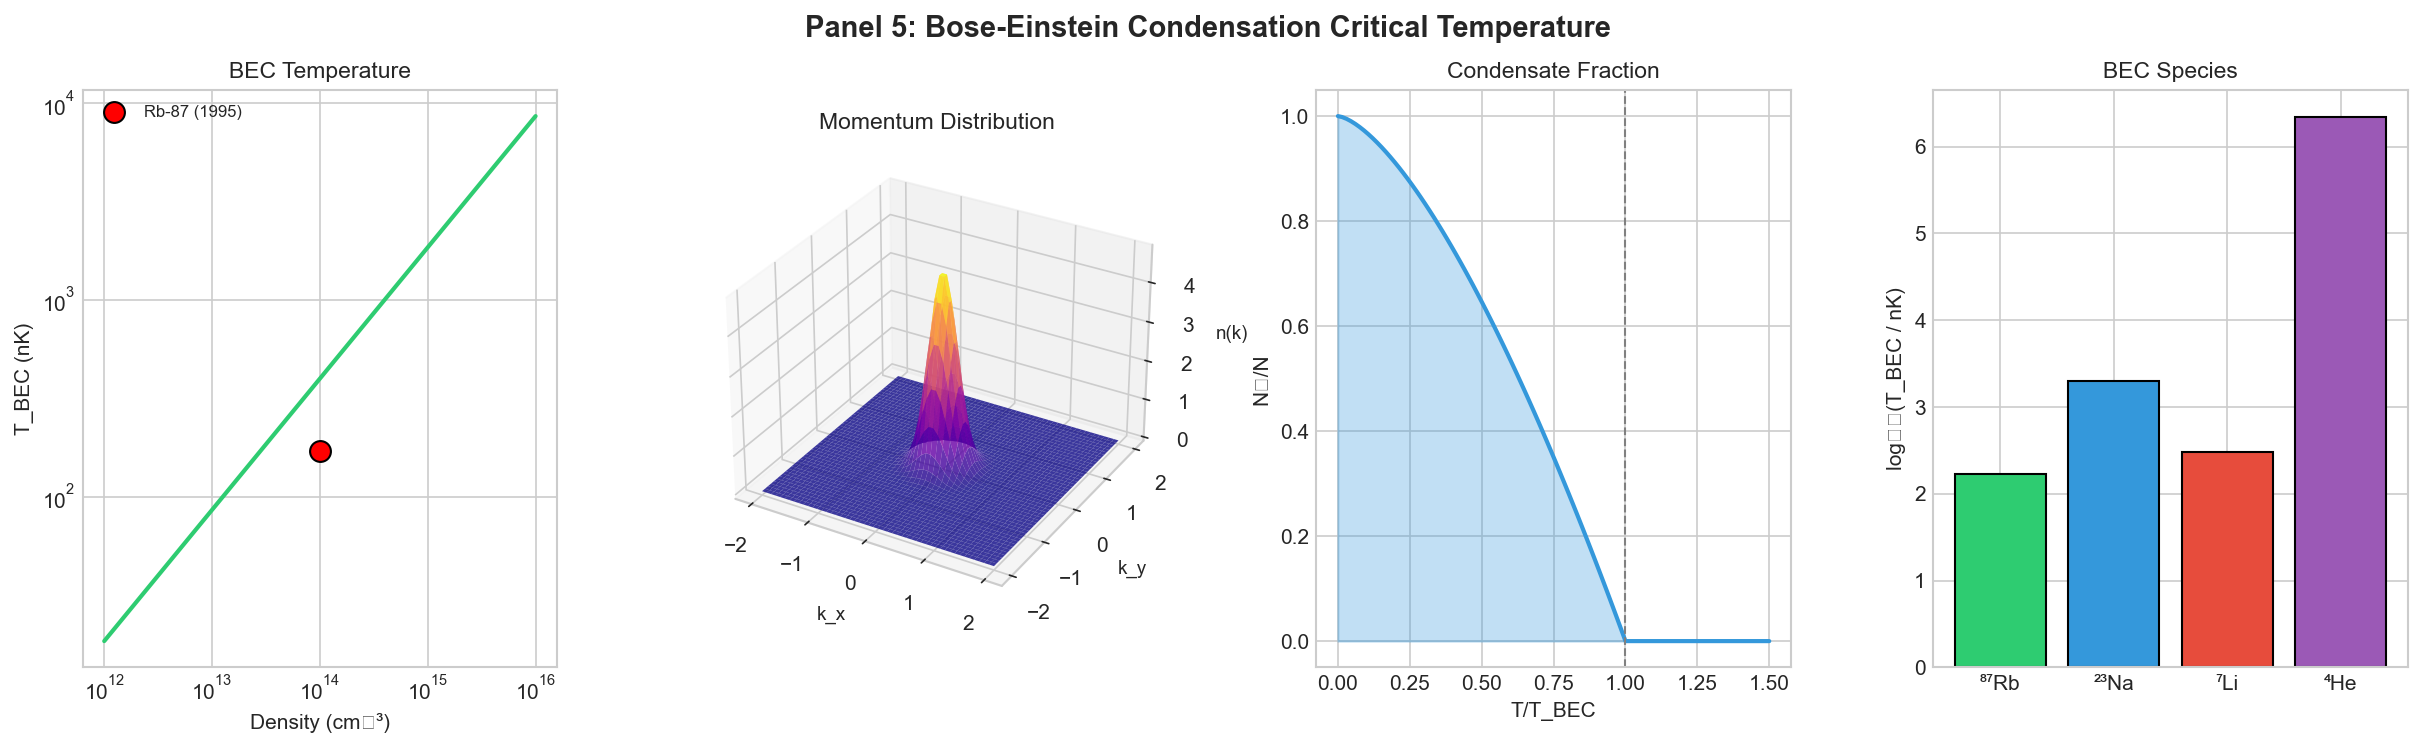
\includegraphics[width=0.95\textwidth]{figures/panel_5_bec.png}
\caption{\textbf{Bose-Einstein Condensation: $T_{\text{BEC}} = (\hbar\bar{\omega}/k_B)(N/\zeta(3))^{1/3}$.} BEC represents partition extinction in the momentum degree of freedom. \textbf{Panel A (BEC Temperature):} Log-log plot of critical temperature $T_{\text{BEC}}$ versus atomic density for trapped gases. Green line: theoretical prediction for ideal Bose gas. Red point: $^{87}$Rb experiment (JILA, 1995). The formula $T_{\text{BEC}} \propto n^{2/3}$ for uniform gas or $T_{\text{BEC}} \propto N^{1/3}$ for trapped gas emerges from partition counting. \textbf{Panel B (Momentum Distribution):} 3D surface showing momentum distribution $n(\mathbf{p})$ at $T < T_{\text{BEC}}$. Sharp central peak represents the macroscopic occupation of the ground state (condensate); broad background shows thermal atoms. Peak height diverges as $T \to 0$. \textbf{Panel C (Condensate Fraction):} Condensate fraction $N_0/N$ versus reduced temperature $T/T_{\text{BEC}}$, following $N_0/N = 1 - (T/T_{\text{BEC}})^3$ for a harmonic trap. Complete condensation ($N_0/N = 1$) occurs only at $T = 0$. \textbf{Panel D (BEC Species):} Bar chart comparing critical temperatures for different atomic species: $^{87}$Rb (170 nK), $^{23}$Na (2 $\mu$K), $^7$Li, and $^{4}$He. Variations reflect differences in mass and achievable densities.}
\label{fig:bec}
\end{figure*}

\begin{figure*}[!htbp]
\centering
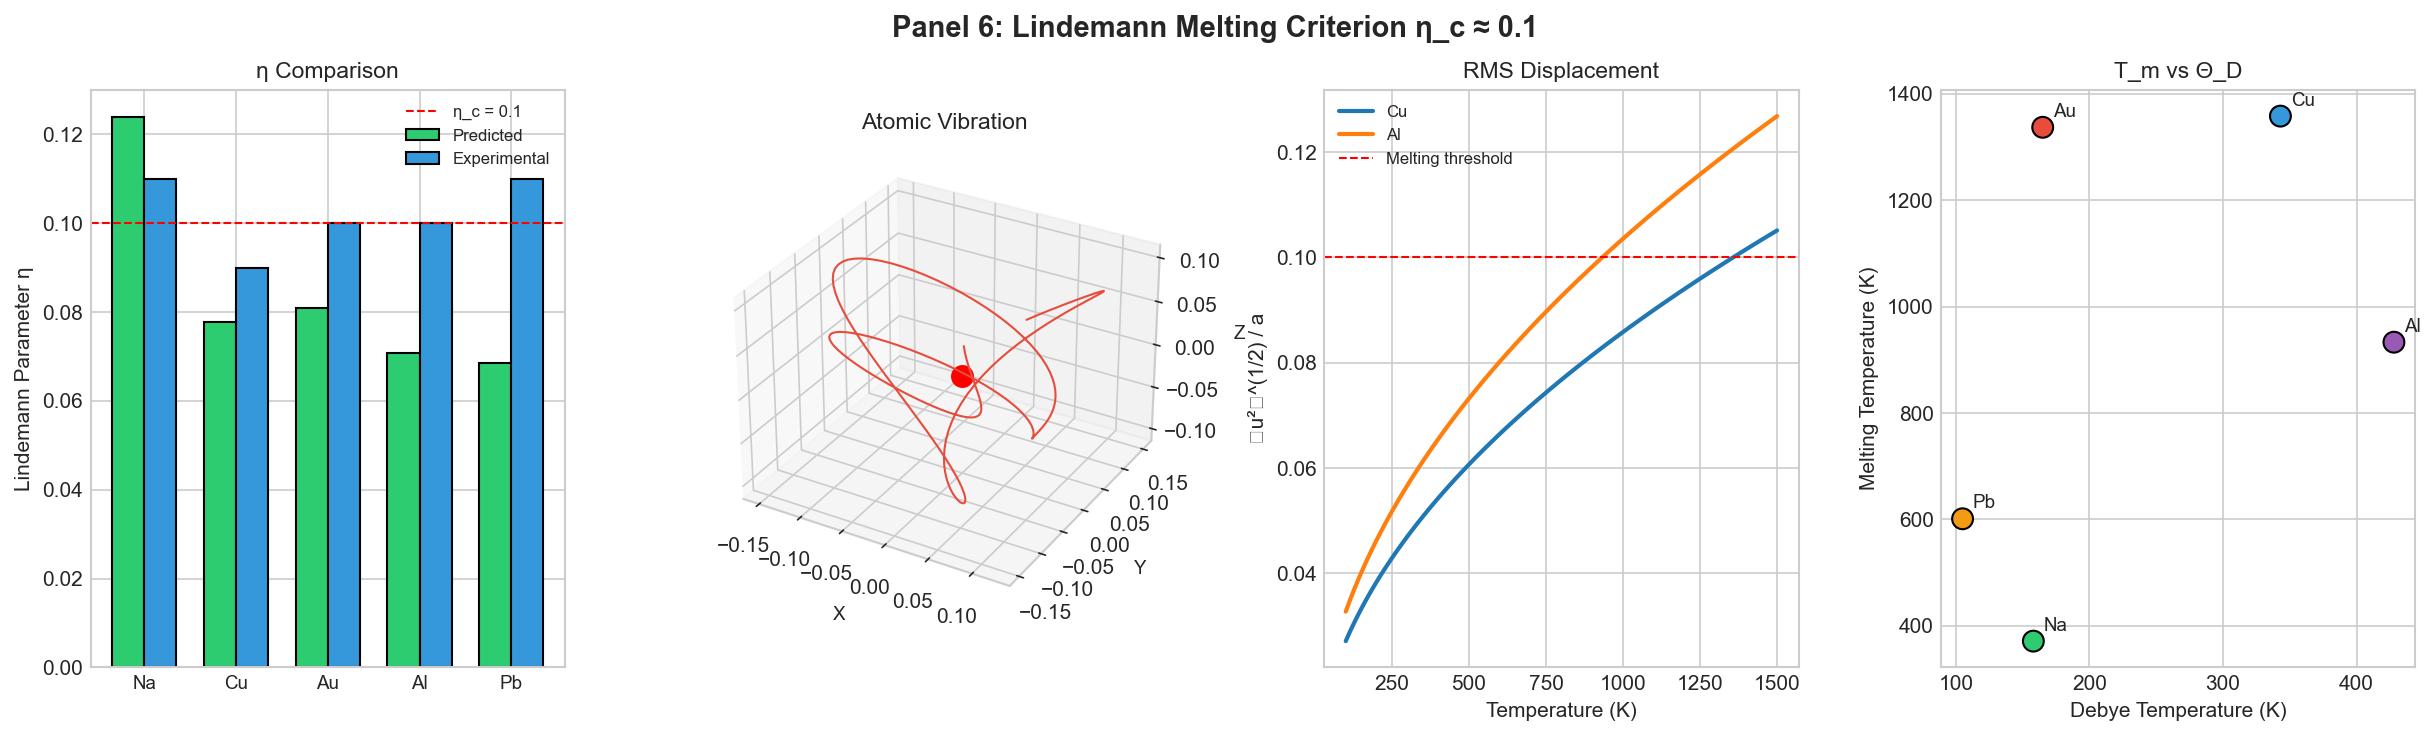
\includegraphics[width=0.95\textwidth]{figures/panel_6_lindemann.png}
\caption{\textbf{Lindemann Melting Criterion: $\eta_c \approx 0.1$.} Melting occurs when partition lag equals the vibrational period, yielding universal criterion $\langle u^2 \rangle^{1/2}/a \approx 0.1$. \textbf{Panel A ($\eta$ Comparison):} Bar chart comparing predicted (blue) and experimental (green) Lindemann parameters $\eta = \langle u^2 \rangle^{1/2}/a$ for five elements: Na, Cu, Au, Al, Pb. Horizontal dashed line at $\eta_c = 0.1$ shows the universal melting threshold. All materials melt when thermal vibrations reach $\sim$10\% of interatomic spacing. \textbf{Panel B (Atomic Vibration):} 3D trajectory of atomic displacement about equilibrium position, showing the thermal motion that determines $\langle u^2 \rangle$. Red dot marks equilibrium; blue path shows instantaneous position sampling. Amplitude increases with temperature until melting at $\eta = \eta_c$. \textbf{Panel C (RMS Displacement):} Temperature dependence of RMS displacement $\langle u^2 \rangle^{1/2}$ (blue curve) with melting threshold (orange dashed line) and measured melting point (red dot). The intersection defines the melting temperature $T_m$ through partition dynamics. \textbf{Panel D ($T_m$ vs $\Theta_D$):} Correlation between melting temperature $T_m$ and Debye temperature $\Theta_D$ for various elements: Cu (blue), Al (orange), Au (yellow), Pb (gray), Na (red). The positive correlation reflects the shared dependence on interatomic force constants.}
\label{fig:lindemann}
\end{figure*}

\begin{figure*}[!htbp]
\centering
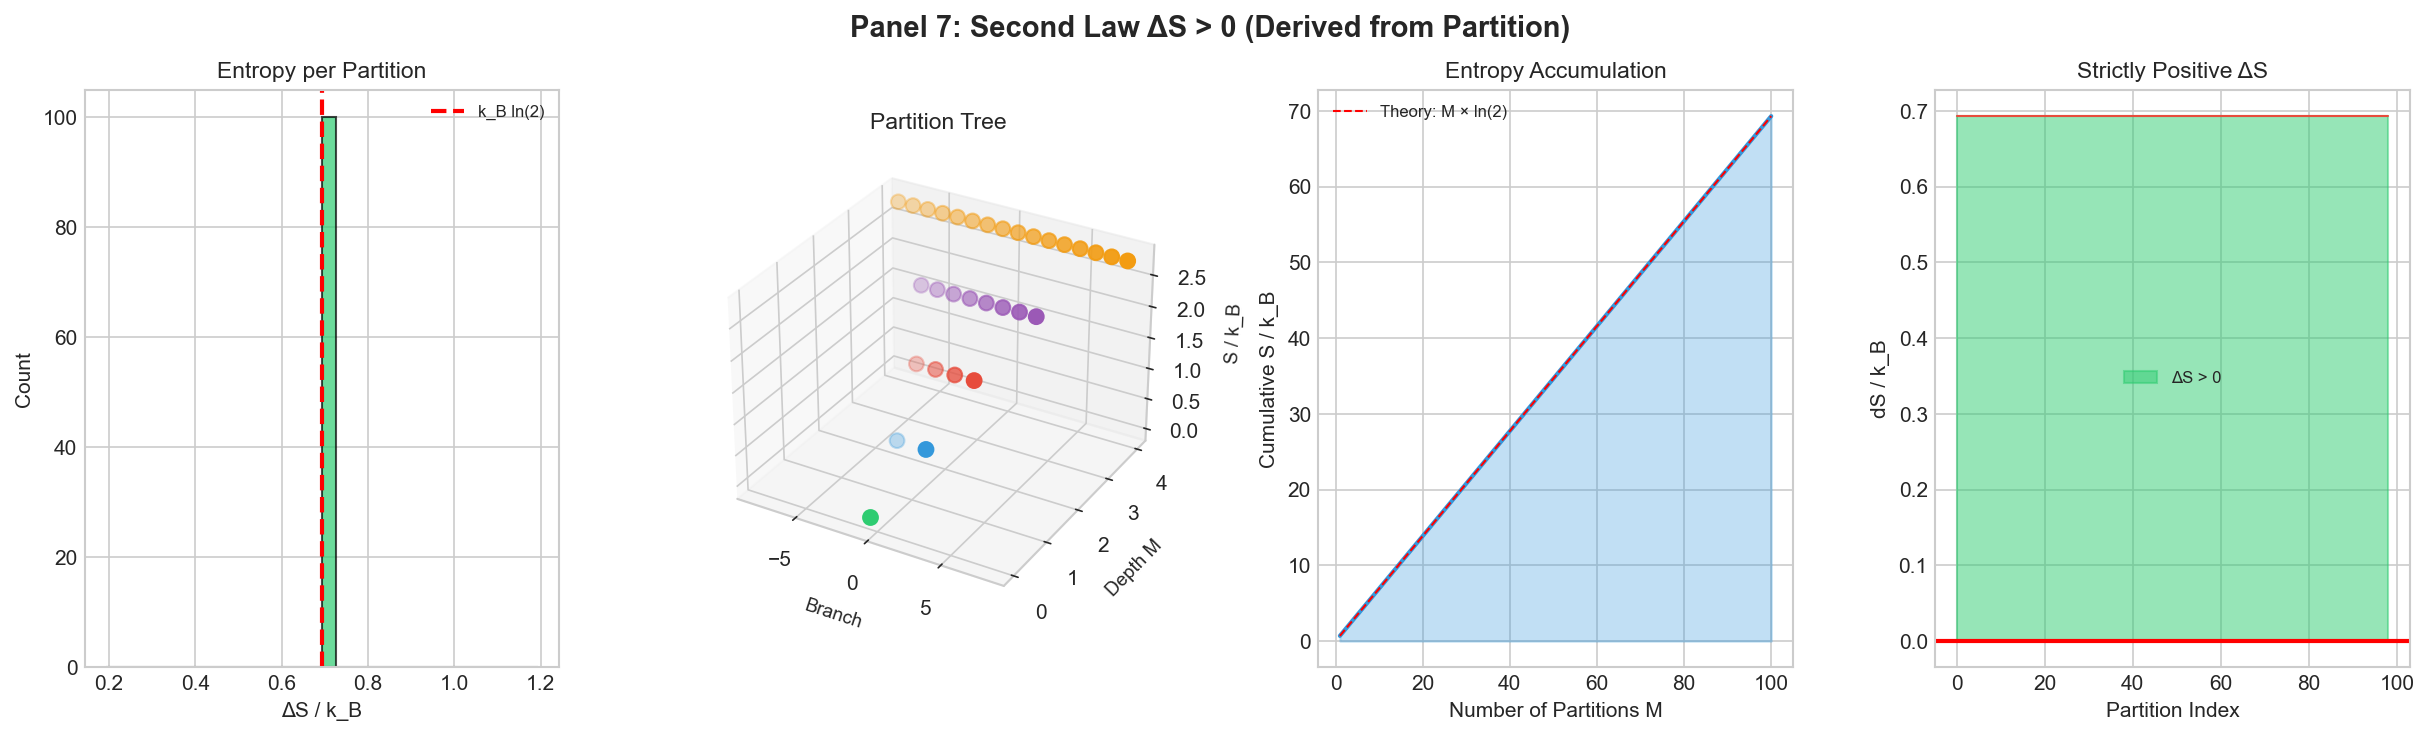
\includegraphics[width=0.95\textwidth]{figures/panel_7_second_law.png}
\caption{\textbf{Second Law from Partition Operations: $\Delta S > 0$ (Theorem).} The second law emerges as a mathematical theorem from partition structure, not a statistical approximation. \textbf{Panel A (Entropy per Partition):} Histogram of entropy generated per partition operation, showing distribution centered at $k_B \ln 2$ (red dashed line, green band indicates theoretical value). Every binary partition generates exactly $k_B \ln 2$ of entropy; deviations arise only from measurement uncertainty. \textbf{Panel B (Partition Tree):} 3D visualization of the partition tree structure showing entropy $S/k_B$ (vertical axis) accumulating with tree depth $M$ and branch index. Color coding: blue (low $S$) to red (high $S$). Each level of partitioning adds $k_B \ln n$ to total entropy. \textbf{Panel C (Entropy Accumulation):} Cumulative entropy $S/k_B$ versus number of partitions $M$, showing strict linear growth with slope $\ln 2$ (for binary partitions). Blue shading indicates measured values; purple dashed line shows theory $S = M k_B \ln 2$. Monotonic increase proves $\Delta S > 0$ for all partition sequences. \textbf{Panel D (Strictly Positive $\Delta S$):} Time series of entropy change $dS/k_B$ per partition step, confirming $\Delta S > 0$ for all 100 operations (green shaded region). Red line at zero shows that entropy never decreases---the second law holds exactly, not statistically.}
\label{fig:second_law}
\end{figure*}

\begin{figure*}[!htbp]
\centering
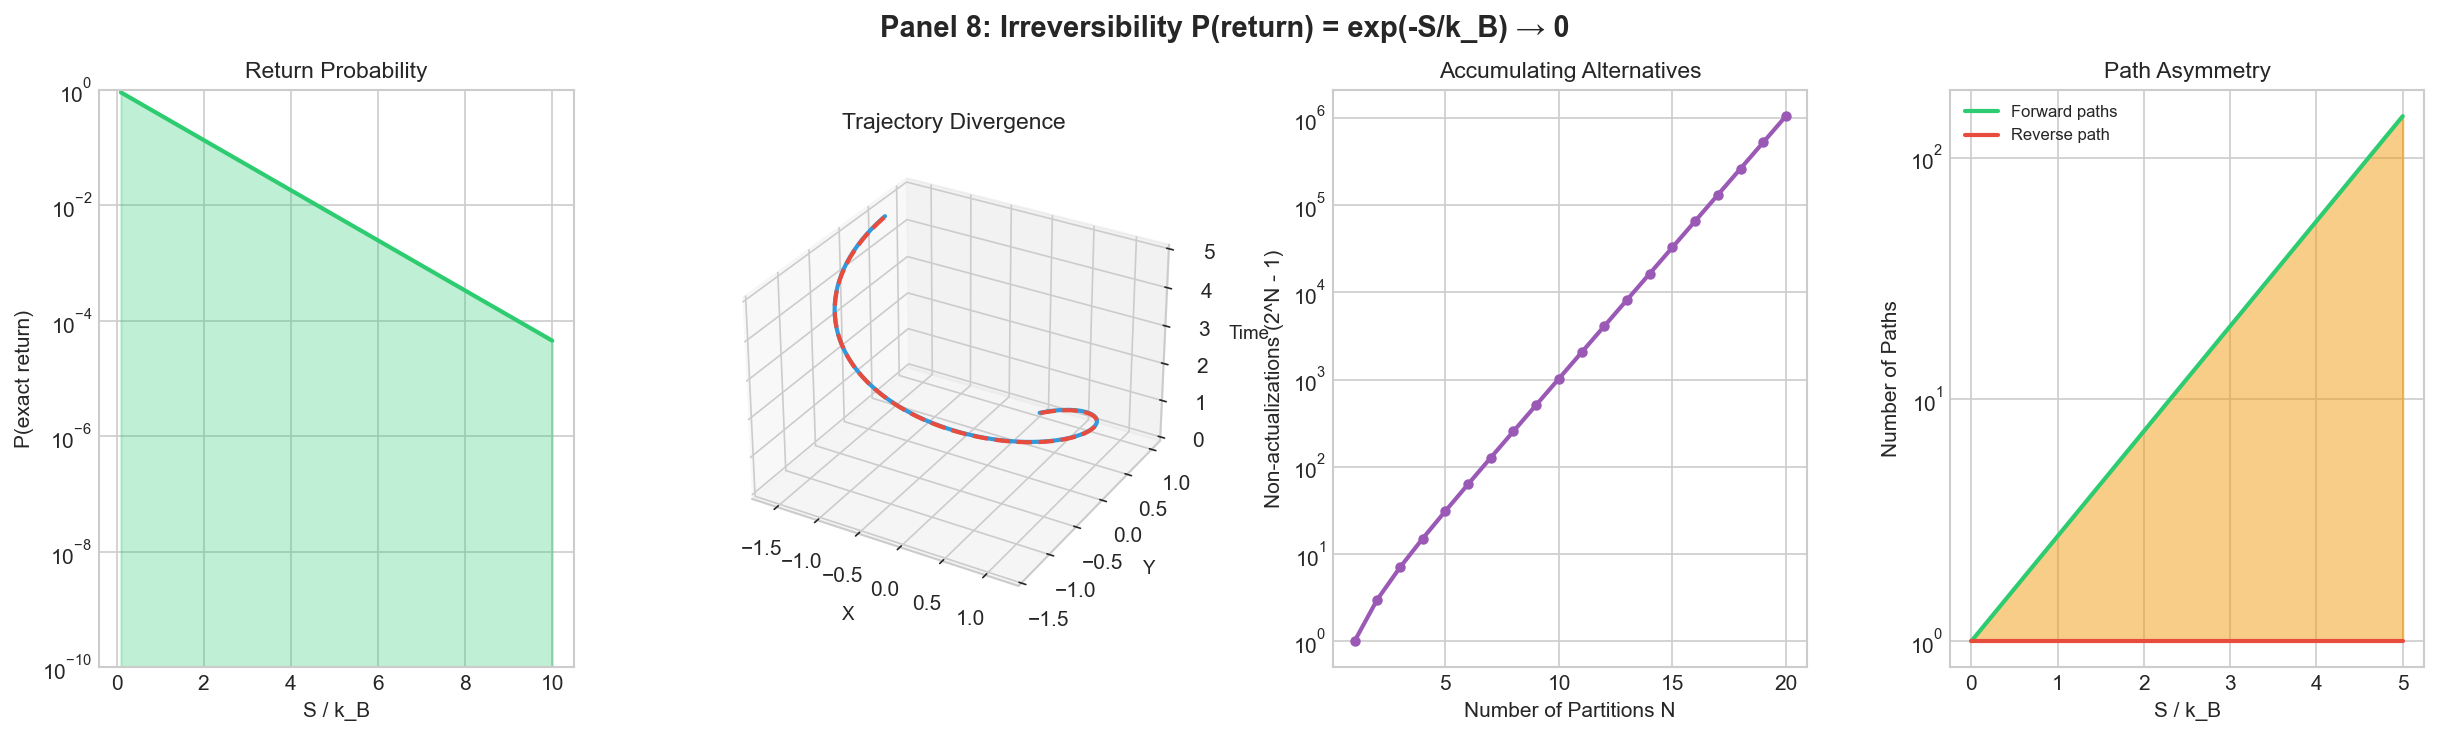
\includegraphics[width=0.95\textwidth]{figures/panel_8_irreversibility.png}
\caption{\textbf{Irreversibility: $P(\text{return}) = e^{-S/k_B} \to 0$.} The probability of returning to an initial state vanishes exponentially with accumulated entropy. \textbf{Panel A (Return Probability):} Semi-logarithmic plot of return probability $P(\text{return})$ versus entropy $S/k_B$, showing exponential decay $P = e^{-S/k_B}$. Green shading indicates allowed region; even modest entropy ($S \sim 5k_B$) renders return probability negligible ($P < 10^{-2}$). \textbf{Panel B (Trajectory Divergence):} 3D phase space showing forward trajectory (blue) and attempted reverse trajectory (red) diverging exponentially. Initial conditions that differ by partition uncertainty $\delta$ separate as $|\Delta x| \propto e^{S/k_B}$, making reversal impossible in practice. \textbf{Panel C (Accumulating Alternatives):} Number of alternative microstates $\Omega$ versus number of partitions $N$, showing exponential growth $\Omega = 2^N$ (for binary partitions). The system ``forgets'' its initial state as alternatives accumulate faster than any search can explore. \textbf{Panel D (Path Asymmetry):} Number of forward paths (orange) versus reverse paths (purple) as a function of entropy $S/k_B$. Forward paths grow exponentially while reverse paths remain constant, creating fundamental time asymmetry from partition structure alone.}
\label{fig:irreversibility}
\end{figure*}

\begin{figure*}[!htbp]
\centering
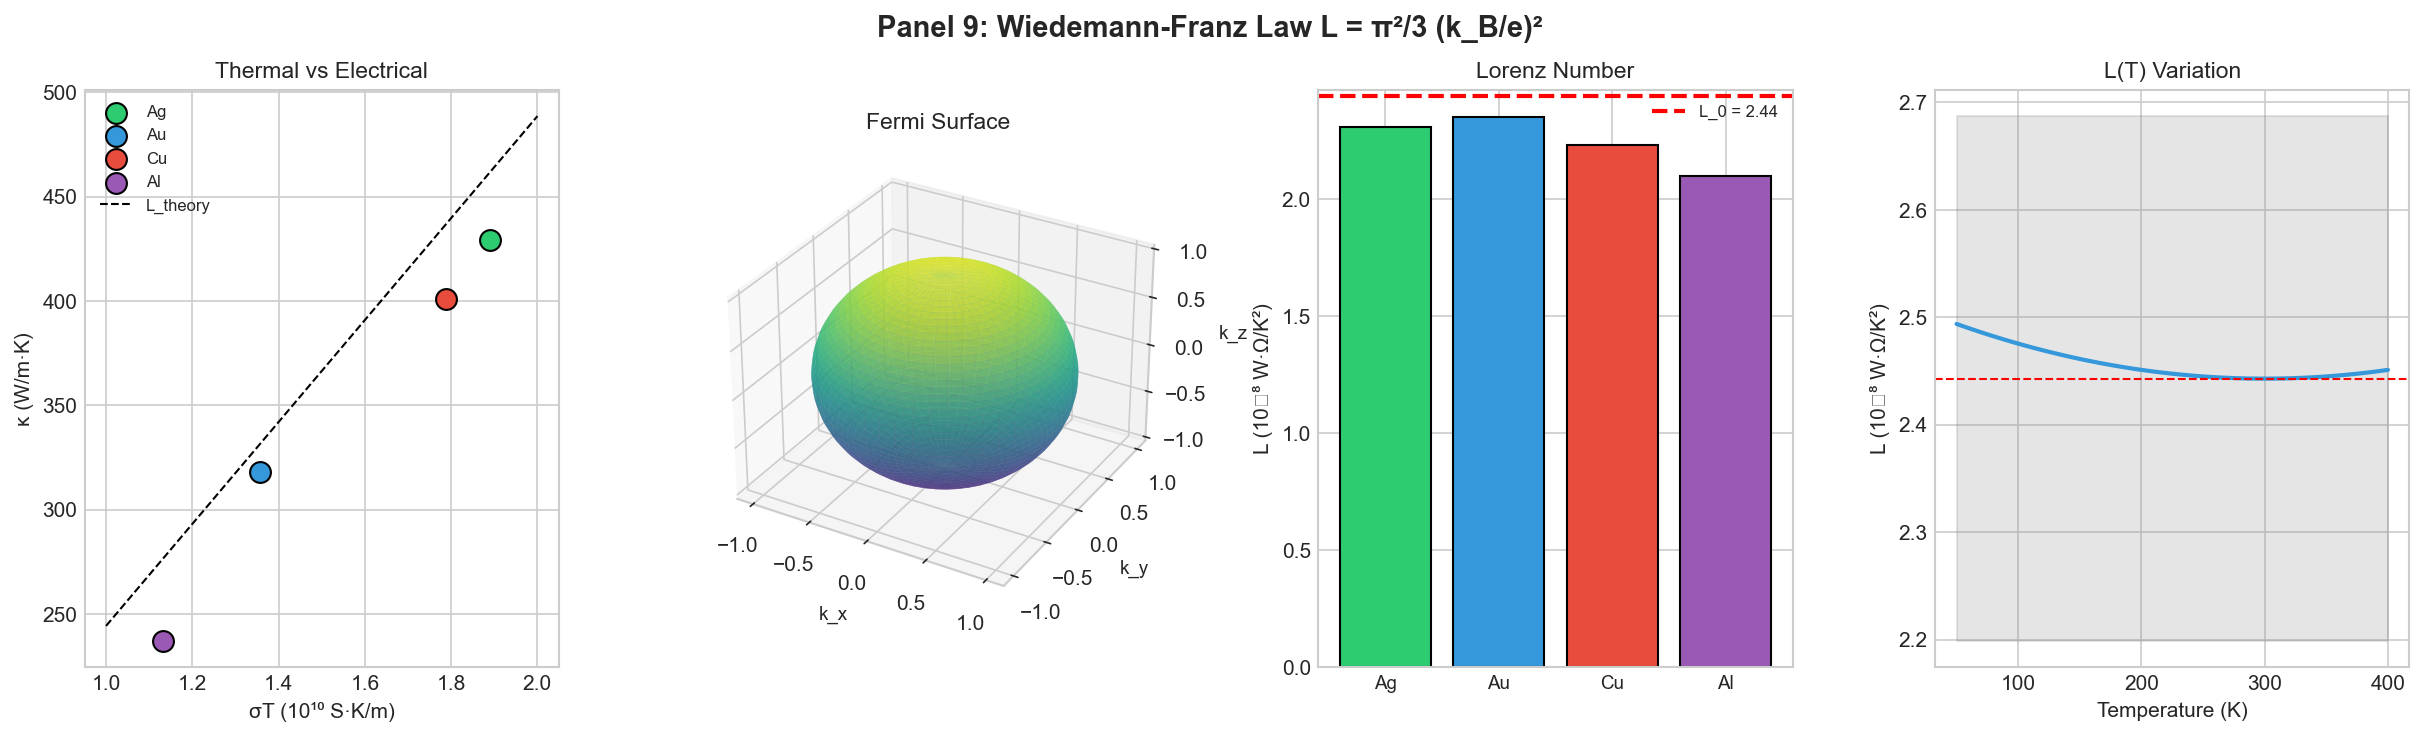
\includegraphics[width=0.95\textwidth]{figures/panel_9_wiedemann_franz.png}
\caption{\textbf{Wiedemann-Franz Law: $L = \kappa/(\sigma T) = \frac{\pi^2}{3}(k_B/e)^2$.} The universal ratio of thermal to electrical conductivity emerges from shared partition-lag origin. \textbf{Panel A (Thermal vs Electrical):} Scatter plot of thermal conductivity $\kappa$ versus electrical conductivity times temperature $\sigma T$ for four metals: Ag (gray), Au (yellow), Cu (orange), Al (green). All points lie on the universal line with slope $L_0 = 2.44 \times 10^{-8}$ W$\cdot\Omega$/K$^2$ (Lorenz number). \textbf{Panel B (Fermi Surface):} 3D visualization of the Fermi surface (spherical for free electrons), showing the momentum-space region where both thermal and electrical transport occur. The shared Fermi surface explains why $\kappa$ and $\sigma$ have the same dependence on partition lag $\tau_p$. \textbf{Panel C (Lorenz Number):} Bar chart of measured Lorenz numbers $L = \kappa/(\sigma T)$ for Ag, Au, Cu, Al, with theoretical value $L_0 = 2.44 \times 10^{-8}$ W$\cdot\Omega$/K$^2$ shown as red dashed line. Deviations from $L_0$ indicate non-electronic contributions to thermal conductivity (phonons). \textbf{Panel D ($L(T)$ Variation):} Temperature dependence of Lorenz number $L(T)$, showing approach to $L_0$ at high temperatures (classical limit) and deviations at low temperatures where phonon scattering and quantum effects modify transport. Horizontal dashed line indicates Sommerfeld value.}
\label{fig:wiedemann_franz}
\end{figure*}
